\documentclass[a4paper, british]{article}

\usepackage[utf8]{inputenc}
\usepackage[T1]{fontenc}
\usepackage{babel}
% \usepackage[margin=2.5cm,a4paper]{geometry}
% \usepackage[skip=1em]{parskip}
\usepackage{lmodern} 
\usepackage{microtype}
% \usepackage{xcolor}
\usepackage{graphicx}
\graphicspath{ {./figures/} }
\usepackage{float}
% \usepackage{enumitem}
\usepackage{adjustbox} % rescale - useful for Dia exported TeX
\usepackage{tikz}
% \usepackage{pgfplots}
\usepackage{booktabs} %tables no vertical lines
% \usepackage{array}
% \usepackage{authblk}
% \usepackage{fancyhdr} %headers and footers
% \usepackage{titlesec}
% \usepackage{tcolorbox} % framed text boxes
% \usepackage{mathtools, amssymb, amsthm}
% \usepackage{gensymb}
\usepackage{chemformula} % chemical formulae
\usepackage{chemfig} % molecular figures
\usepackage{siunitx}
\usepackage{csquotes}
\usepackage[titletoc, title]{appendix}
% \usepackage{lettrine} % initials

\usepackage[
pdfauthor={Adam Menne},
pdftitle={Chemistry 254 - Practical 6},
pdfsubject={},
pdfkeywords={}]{hyperref}

\usepackage[noabbrev]{cleveref}

\usepackage[
backend=biber,
style=numeric,
sorting=none,
doi=true,
isbn=false
]{biblatex}
\addbibresource{citations.bib}

\setlength{\parskip}{1em}
\setlength{\parindent}{0em}
\linespread{1.3}

\title{Chemistry 254\\ Experiment 6\\ First order reactions}
\date{Last edited on \today}
\author{Adam Menne\\ Stellenbosch University}

\begin{document}

\maketitle

\begin{abstract}
\noindent
In this practical the reaction rate of a first order reaction is investigated with a focus on determining the reaction rate constant and half life.
\end{abstract}

\tableofcontents

\newpage


\section{Results}

\begin{figure}[H]
    \centering
    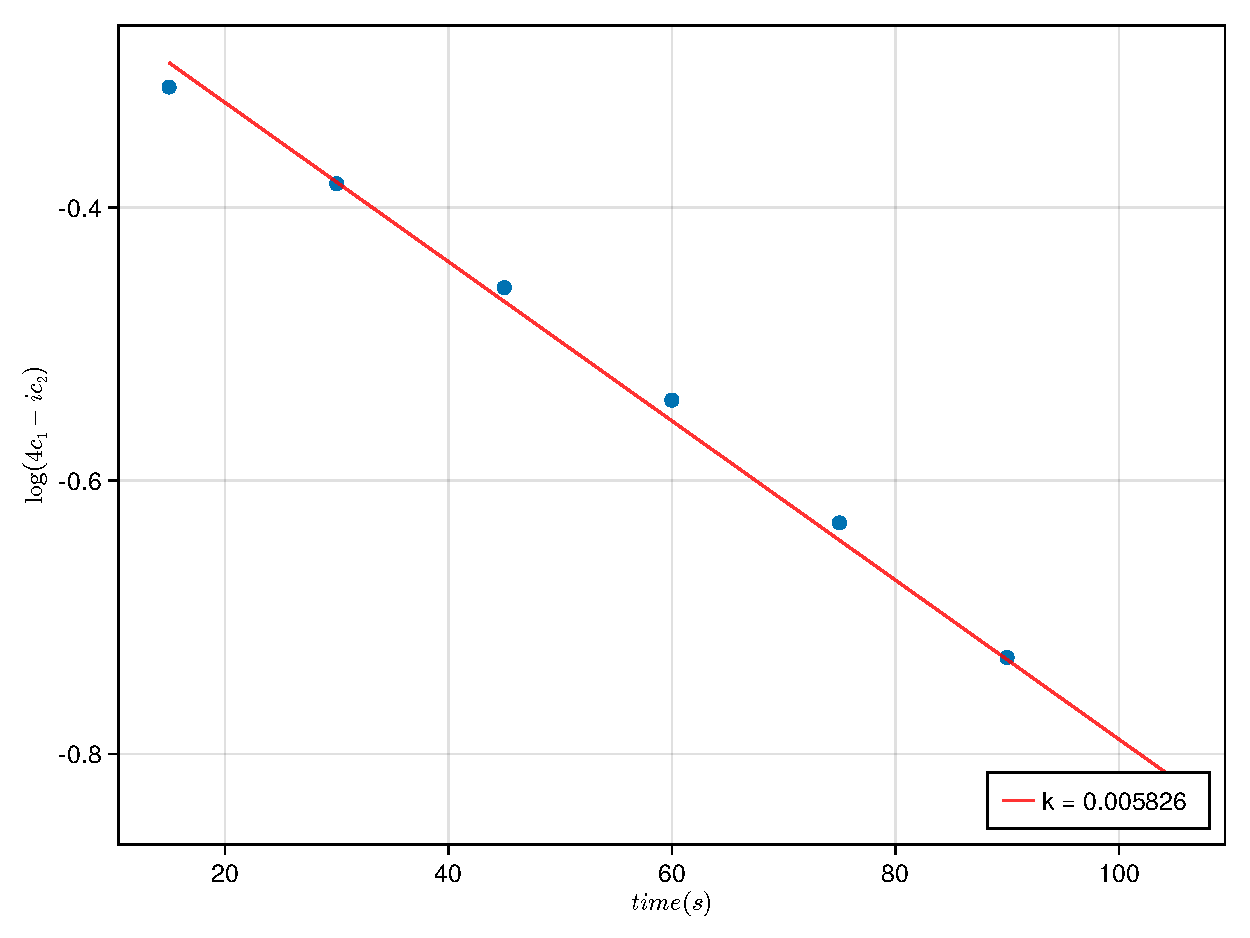
\includegraphics[width=\textwidth]{figures/f1.pdf}
    \caption{\(ln(4c_1 - ic_2)\) over reaction time}
    \label{fig:f1}
\end{figure}

From \cref{fig:f1} the reaction rate constant was determined to be 0.005826

\Cref{tab:k} show the reaction rate constants for all samples with their respective reaction times. The mean value for k 0.004967 with a standard deviation of 0.0004473

\begin{table}[H]
    \centering
    \caption{Reaction rate constants}
    \vspace*{2mm}
    \label{tab:k}
    \begin{tabular}{cc}
    \toprule
    Reaction time & k \\ \midrule
    15 & 0.004403 \\
    30 & 0.004559 \\
    45 & 0.004730 \\
    60 & 0.004920 \\
    75 & 0.005133 \\
    90 & 0.005374 \\
    105 & 0.005648\\
    \bottomrule
    \end{tabular}
\end{table}

The concentration of Hydrogen peroxide was found to be 0.1955 \(M\)

A static export of the notebook containing all analysis and figures is available at \url{https://adammenne.github.io/chemistry_254/practical_6/notebook.html}.\\ With full source code available at \url{https://github.com/AdamMenne/chemistry_254/tree/master/practical_6}

\section{Discussion}

While the k values have relatively low standard deviation they do increase proportionally to reaction time. Notably the value determined using \cref{fig:f1} is slightly higher than the highest value shown in \cref{tab:k}.

Accuracy could be increased with a larger sample size, and a more consistent method of identifying reaction times.

\newpage

\begin{appendices}

\section{MSDS}

\subsection*{Potassium iodide}

\begin{itemize}
    \item Harmful
    \item[-] may cause skin and eye irritation
    \item[-] if in contact with skin or eyes wash for several minutes 
\end{itemize}

\subsection*{Sodium thiosulfate}

\begin{itemize}
    \item Harmful
    \item[-] causes skin, eye, and respiratory irritaion
    \item[-] if in contact with skin or eyes wash for several minutes  
\end{itemize}

\subsection*{Acetic acid}

\begin{itemize}
    \item Flammable, corrosive
    \item[-] causes skin burns and eye damage
    \item[-] if in contact with skin or eyes wash for several minutes  
\end{itemize}

\subsection*{Hydrogen peroxide}

\begin{itemize}
    \item Oxidising, corrosive, harmful
    \item[-] do not ingest or inhale
    \item[-] may cause skin burns, eye damage
    \item[-] if in contact with skin or eyes wash for several minutes  
\end{itemize}

\end{appendices}

\end{document}